\section{Task 2}

\subsection{Breakdown of the memory errors \% in Single, dual, triple, quadruple bit errors}

To determine the number of bits in a memory error, we looked up the
corresponding syndrome in the syndrome table.  Once the entry is located, we
check the error bitmask and count the number of `1's in the bitmask.  This
number tells us the number of bits in error when that syndrome was
reported\cite{AMD_BKDG}.  We calculated the number of bits per error for all
memory errors, gathered results and calculated the distribution across machine
type. The results of this study are presented in Table \ref{tab:mem_breakdown}

% latex table generated in R 3.0.2 by xtable 1.7-1 package
% Sun Mar  2 01:04:22 2014
\begin{table}[ht]
\centering
\caption{Memory Error Percentage Breakdown by number of bits and machine type}
\label{tab:mem_breakdown}
\begin{tabular}{rrrrrrr}
  \hline
 & compute & GPU & lnet & service & mom & ALL \\
  \hline
1 & 86.79 & 92.09 & 100.00 & 99.87 & 82.00 & 89.72 \\
  2 & 5.48 & 2.36 & 0.00 & 0.13 & 18.00 & 4.28 \\
  3 & 2.18 & 0.84 & 0.00 & 0.00 & 0.00 & 1.66 \\
  4 & 2.51 & 3.20 & 0.00 & 0.00 & 0.00 & 2.02 \\
  5+ & 3.03 & 1.52 & 0.00 & 0.00 & 0.00 & 2.32 \\
   \hline
\end{tabular}
\end{table}

From table \ref{tab:mem_breakdown}, we can make a few important observations regarding the data:
\subsubsection{Multibit errors are significant:} Roughly 10\% of all memory
errors are multibit errors.  It should also  

\subsubsection{Chipkill is extremely effective:}  There was only one
uncorrectable memory error in our dataset, but there were 11633 corrected
errors.  Again, 10\% of those were multibit and were therefore corrected.  If
the behavior exhibited during these 8 days was representative of a year, we
could expect around 55,000 multibit errors per year. Having that many
uncorrectable errors in a year would be unacceptable in nearly any environment
(except perhaps a stateless web server farm).  Therefore, Chipkill is not only
beneficial for a system like Blue Waters, but necessary.

\subsubsection{Compute nodes exhibit the largest percentage of multibit
errors:} While compute nodes had a lower percentage of multibit errors (on
average) in our dataset, it is difficult to tell if that trend would extend
across the full dataset.  Since GPU and service nodes have half of the DIMMs
present in compute nodes, the number of multibit errors may be undersampled in
our eight day dataset.

\subsection{How frequent (time) are multiple (>1) bit errors?}

Fig. \ref{fig:mem_error_per_hr} plots the number of memory errors per hour for
each machine type.  In this figure, it is easy to see that memory errors in 
compute nodes clearly dominate.  However, this trend could be attributed to the
large number of compute nodes (22640) compared to the fewer GPU (4192) and
service (1936) nodes.  Therefore, this figure was normalized to the number of
node types in Fig. \ref{fig:mem_error_per_hr_normed}.  In this plot, all of the
rates differ by orders of magnitude.  For such a small dataset, it is easy for a
few nodes to dominate.  However, one could still expect different node types to
behave differently as all of these types differ in the way they use memory.

\begin{figure}[h]
  \centering
  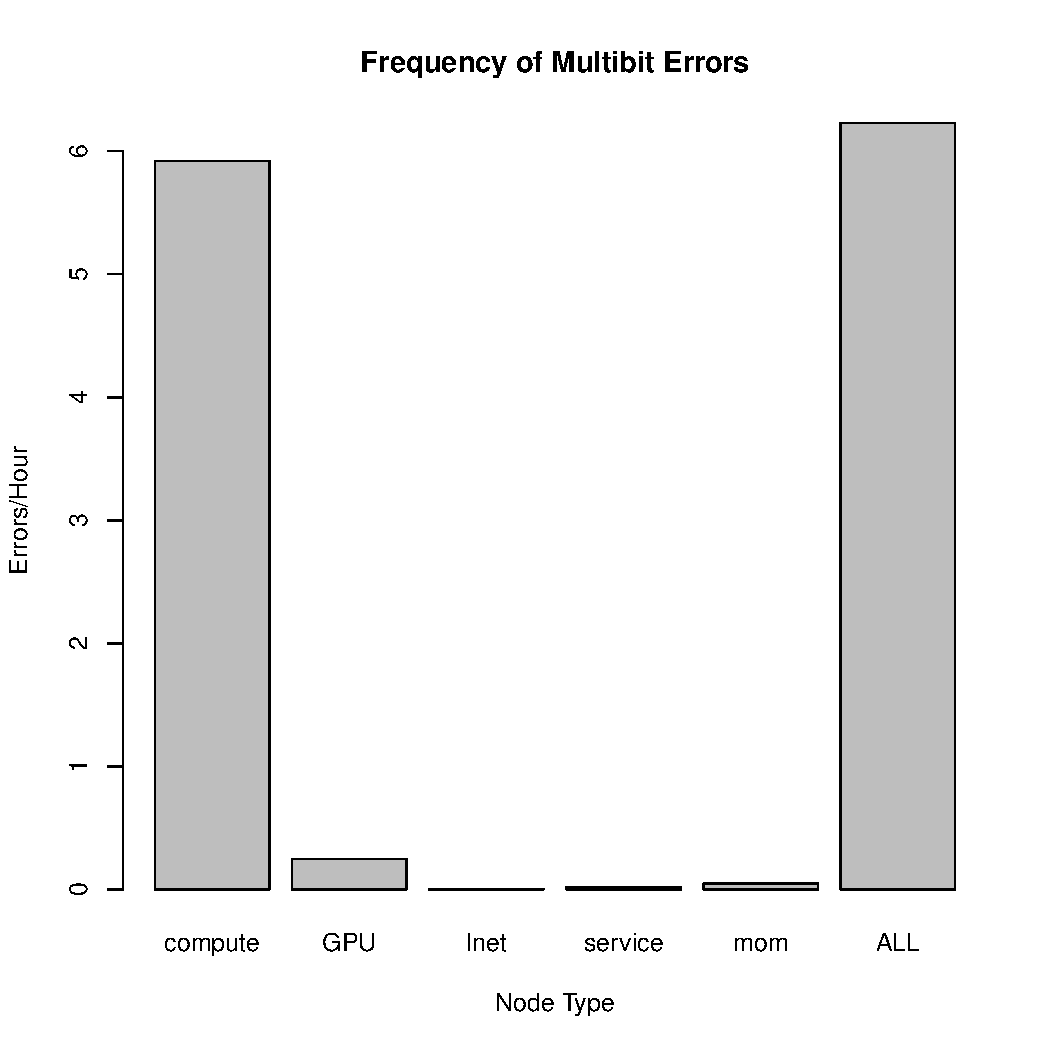
\includegraphics[width=0.45\textwidth]{images/task2_2}
  \caption{Bar graph for the number of Memory errors/hour for each machine
  type.}\label{fig:mem_error_per_hr}
\end{figure}

\begin{figure}[h]
  \centering
  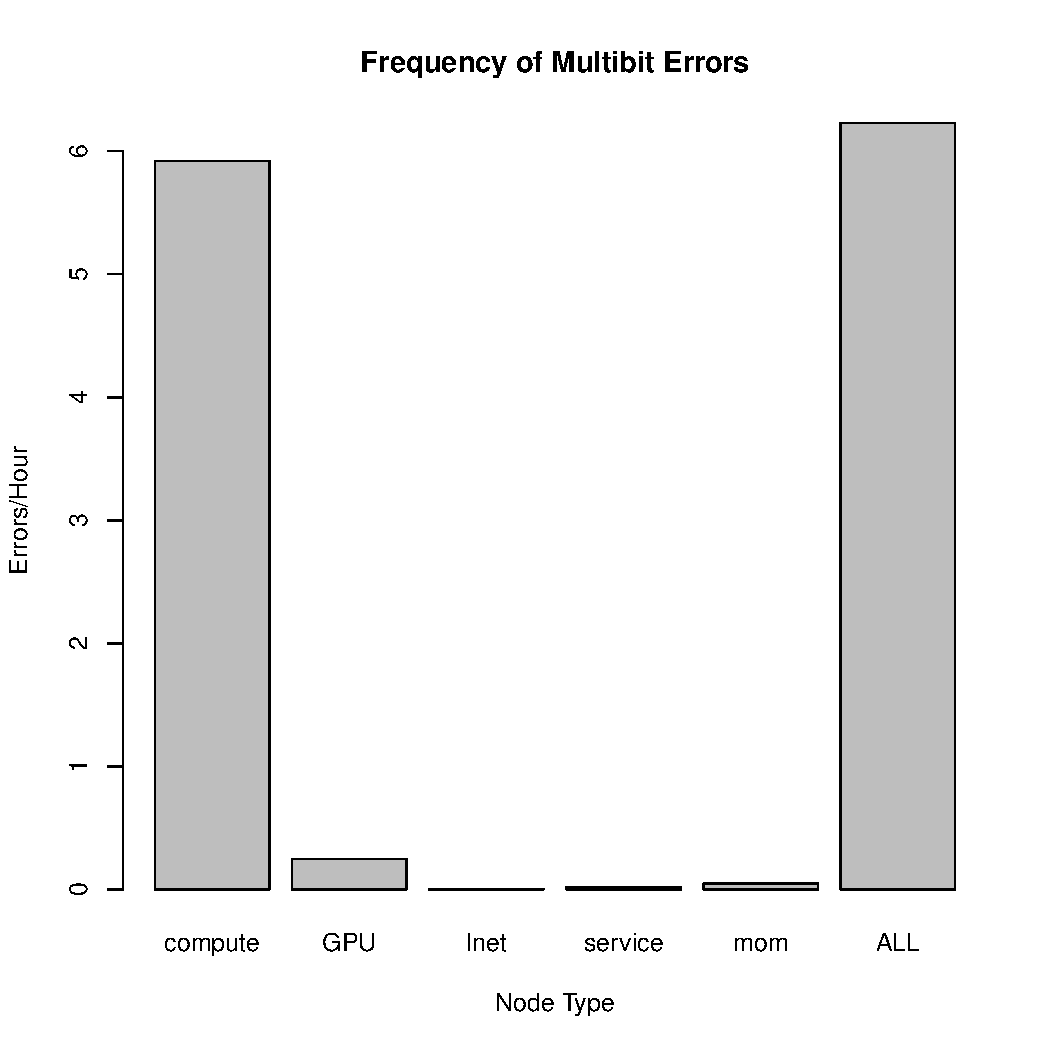
\includegraphics[width=0.45\textwidth]{images/task2_2}
  \caption{Bar graph for the number of Memory errors/hour for each machine
  type, normalized to the number of nodes in each
  type.}\label{fig:mem_error_per_hr_normed}
\end{figure}

\subsection{How many uncorrectable errors would Blue Waters have if using only ECC? How effective is Chipkill wrt ECC?}

If Blue Waters had only ECC, it would not be able to correct any multibit
errors, so errors in more than one bit would become uncorrectable.  There were
1196 errors that would have become uncorrectable without Chipkill.  This makes
Chipkill extremely effective and the data here present a strong case for
Chipkill being mandatory in a system of this size.

A table comparing the same system with and without Chipkill is shown in Table
\ref{tab:mem_fit_mtbf}.
\begin{table}[ht]
\centering
  \begin{tabular}{rrr}
  \hline
  & FIT/Mbit & MTBF \\ 
  \hline
  Chipkill & 0.00039 & 192.00 \\ 
  No Chipkill & 0.47150 & 6.23 \\ 
  \hline
\end{tabular}
\caption{FIT/Mbit and MTBF. One FIT = 1 Failure in $10^9$ hours, MTBF is in
hours.}
\label{tab:mem_fit_mtbf}
\end{table}

In Table \ref{tab:mem_fit_mtbf}, we present the MTBF and FIT/Mbit for Blue
Waters given our dataset.  Again, Chipkill demonstrates its value and is
indispensable for a system of this size.   Here, we present FIT/Mbit so that
we can compare with the study in \cite{schroeder2009dram}.  To calculate
FIT/Mbit, we counted the number of uncorrectable errors (with and without
Chipkill) and used the following formula:
\begin{equation*}
  FIT = \frac{10^9N_{\textrm{failures}}}{(1614080\cdot8\cdot1024)t}
\end{equation*}
, where $t=8*24$ is the timespan of the data set in hours and the system has
1614080GiB of memory and there are $8\dot1024$ GiB to a Mbit. In the
aforementioned study, the authors found an average of 778--25,000 FIT/Mbit for
their systems (ECC only DDR DIMMs).  The values calculated here are
significantly, but the authors of \cite{schroeder2009dram} cite that previous
lab studies showed DRAM to exhibit < 1 FIT/Mbit.  The MTBF without Chipkill
becomes significantly smaller since with Chipkill there was only one
uncorrectable error.
